\documentclass{svproc}

% -----------------------------------------------------------------------------
% Draft for Complex Networks and their Applications 2026
% Working conference-paper version reshaped from the graph-curvature project.
% Replace llncs.cls with the official Springer template if the conference package differs.
% -----------------------------------------------------------------------------

\usepackage[T1]{fontenc}
\usepackage{graphicx}
\usepackage{multirow}
\usepackage{amsmath,amssymb,amsfonts}
\usepackage{mathrsfs}
\usepackage{xcolor}
\usepackage{textcomp}
\usepackage{booktabs}
\usepackage{url}
\def\UrlFont{\rmfamily}
\graphicspath{{results/figures/}}
\emergencystretch=2em

\title{Shortest-Path Anisotropy as a Graph Diagnostic for Curvature Organization in Sampled Geometries}
\titlerunning{Shortest-Path Anisotropy in Sampled Geometries}

\author{Ariadna Uxue Palomino Ylla}
\authorrunning{A. U. Palomino Ylla}
\institute{Nagoya University, Nagoya, Japan\\
\email{ariadnauxue@gmail.com}}

\begin{document}
\mainmatter
\maketitle

\begin{abstract}
Spatial graphs built from sampled geometric domains encode information about the underlying space through their connectivity and shortest-path structure. However, separating genuine geometric organization from artifacts of sampling density, graph construction, or boundary effects remains a central difficulty. We introduce a shell-based shortest-path anisotropy statistic designed to quantify how unevenly shortest-path multiplicities are distributed around a source node at fixed graph distance. For a graph radius $r_g$, the statistic compares the logarithmic number of graph shortest paths from a source node to all nodes in the graph shell $S_{r_g}(p)$, producing a local diagnostic $C_{\log}(p,r_g)$. We evaluate the method on matched graph discretizations of flat, hyperbolic, and black-hole-inspired geometries, with particular focus on Flamm--Schwarzschild spatial slices. In this benchmark, the Schwarzschild Kretschmann scalar $K_{\mathrm{Schw}}$ provides a monotonic continuum reference profile associated with the parent spacetime geometry. In radial-binned experiments, the proposed statistic exhibits a strong monotonic relation with curvature organization, including a correlation of approximately $0.91$ with $\log K_{\mathrm{Schw}}$ in the Flamm benchmark, while matched-flat controls do not reproduce the same systematic radial trend. Refinement tests show improved rank agreement as the number of sampled points is increased. These results support shortest-path anisotropy as a curvature-sensitive graph diagnostic for sampled spatial networks. The method is not proposed as a graph-independent continuum curvature invariant; rather, it is a calibrated network measure for detecting geometric organization under a specified graph-construction protocol.

\keywords{Spatial networks, shortest paths, graph geometry, curvature diagnostics, complex networks, sampled manifolds}
\end{abstract}

\section{Introduction}

Spatial networks arise whenever data points are embedded in, sampled from, or constrained by an underlying geometric domain. Examples include transportation networks, sensor networks, biological transport systems, spatial proximity graphs, discretized physical spaces, and geometric graphs used in numerical and computational modeling. In such settings, the graph is not only an abstract combinatorial object: its connectivity may retain information about the geometry from which it was generated. A central question is therefore how much geometric organization can be recovered from graph observables alone.

This question is especially subtle when the graph is obtained from a finite sampling of a curved space. Local degree, clustering, path length, and graph curvature measures can change not only because the underlying geometry changes, but also because of sampling density, boundary truncation, finite-size effects, and the chosen graph-construction rule. Consequently, a useful graph diagnostic should be tested against matched controls and interpreted as part of a calibrated graph-discretization protocol rather than as an automatic replacement for continuum curvature.

In this work, we introduce a shortest-path anisotropy statistic for spatial graphs sampled from geometric domains. The basic idea is simple. Around a source node $p$, consider all nodes at a fixed graph distance $r_g$. If the graph is locally homogeneous and isotropic, the multiplicities of shortest paths from $p$ to this shell should vary in a relatively balanced way. In a graph discretization of a radially organized curved geometry, by contrast, the distribution of shortest-path multiplicities may become directionally uneven. We quantify this unevenness through a logarithmic cubic-mean-deviation statistic, denoted $C_{\log}(p,r_g)$.

The method is motivated by the observation that path multiplicity is a sensitive probe of graph geometry. Unlike a single shortest-path distance, the number of shortest paths captures degeneracy: it records how many equivalent minimal routes connect two nodes. Curved or radially distorted graph discretizations can break or reorganize this degeneracy. Instead of assigning curvature directly to edges or nodes, our statistic measures the anisotropy of shortest-path multiplicities on shells. This makes it complementary to existing graph-curvature constructions such as Forman--Ricci and Ollivier--Ricci curvature.

We benchmark the statistic on graph discretizations of flat, hyperbolic, and black-hole-inspired spatial geometries. The main case study is a Flamm--Schwarzschild spatial slice. For this benchmark, the Schwarzschild Kretschmann scalar provides a monotonic continuum reference profile associated with the parent Schwarzschild geometry:
\begin{equation}
K_{\mathrm{Schw}}(r)=\frac{48M^2}{r^6}.
\end{equation}
We do not claim that the graph statistic reconstructs this scalar directly. Rather, we use $K_{\mathrm{Schw}}(r)$ as an external radial reference to test whether a graph-only shortest-path statistic detects the same organized radial structure after controlling for sampling and construction effects.

Our contributions are as follows:
\begin{enumerate}
    \item We define a shell-based shortest-path anisotropy statistic for spatial graphs, based on the logarithmic dispersion of shortest-path multiplicities.
    \item We present a matched-control protocol for separating curvature-related organization from sampling artifacts.
    \item We evaluate the statistic on flat, hyperbolic, and black-hole-inspired graph discretizations, with a detailed Flamm--Schwarzschild benchmark.
    \item We show that the statistic tracks radial curvature organization in the curved benchmark while remaining comparatively weak or inconsistent in matched-flat controls.
\end{enumerate}

\section{Related Work}

Graph-based notions of geometry have a long history in network science, discrete differential geometry, and mathematical physics. Curvature on graphs is often studied through local or edge-based quantities. Forman--Ricci curvature adapts ideas from discrete Morse theory to cell complexes and has been widely used as a computationally efficient network curvature measure. Ollivier--Ricci curvature compares probability measures transported along graph edges and is closely related to optimal transport and metric-measure geometry. Both measures have found applications in network robustness, community structure, biological networks, and geometric data analysis.

The present work follows a different but complementary direction. Instead of defining an edge curvature, we consider the distribution of shortest-path multiplicities from a node to a fixed graph shell. This is closer in spirit to studying how families of graph shortest paths expand, focus, or become directionally organized in a discretized geometry. The statistic is therefore not a competitor to Forman--Ricci or Ollivier--Ricci curvature in a strict sense. It measures a different object: anisotropy in the degeneracy of shortest paths.

The method is also related to the broader study of spatial networks and geometric graphs. In spatial networks, graph structure is constrained by embedding, distance, and domain geometry. In random geometric graphs and nearest-neighbor graphs, small changes in sampling or metric structure can affect connectivity and shortest paths. This motivates the use of matched controls in our experiments. A raw graph statistic is rarely meaningful by itself; it must be compared against graphs with similar sampling, size, and construction rules.

Finally, the use of black-hole-inspired spatial slices as benchmark geometries connects the method to discretized approaches in gravitational physics. Here, however, the physical geometry is used primarily as a controlled test bed for graph diagnostics. The target audience of this paper is network science: the central object is a graph statistic, and the physical geometry supplies an interpretable benchmark with a known radial curvature profile.

\section{Method}

\subsection{Spatial Graph Construction}

Let $\mathcal{M}$ be a geometric domain from which points are sampled. Each sampled point becomes a node in a graph $G=(V,E)$. Edges are then added according to a fixed graph-construction rule, such as a $k$-nearest-neighbor rule in the embedded metric or in the coordinate representation used for the benchmark. We denote by $d_G(p,q)$ the shortest-path distance between two nodes $p,q\in V$ in the unweighted graph.

The experiments in this paper use matched graph construction across geometries. That is, when comparing a curved geometry to a flat control, we keep the number of sampled nodes, graph-construction rule, graph-radius range, and random-seed protocol as similar as possible. This is essential because shortest-path statistics are sensitive to graph density and sampling irregularities.

\subsection{Graph Shells and Shortest-Path Multiplicity}

For a node $p\in V$ and an integer graph radius $r_g\geq 1$, define the graph shell
\begin{equation}
S_{r_g}(p)=\{q\in V: d_G(p,q)=r_g\}.
\end{equation}
The corresponding graph ball is
\begin{equation}
B_{r_g}(p)=\{q\in V: d_G(p,q)\leq r_g\}.
\end{equation}

For every target node $q\in S_{r_g}(p)$, let
\begin{equation}
N_{\mathrm{geo}}(p,q)
\end{equation}
be the number of shortest paths from $p$ to $q$. This quantity is at least one for nodes in the same connected component. Shortest-path multiplicity contains more information than shortest-path distance alone. While $d_G(p,q)$ gives the length of a minimal route, $N_{\mathrm{geo}}(p,q)$ measures the degeneracy of minimal routes.

\begin{figure}
\centering
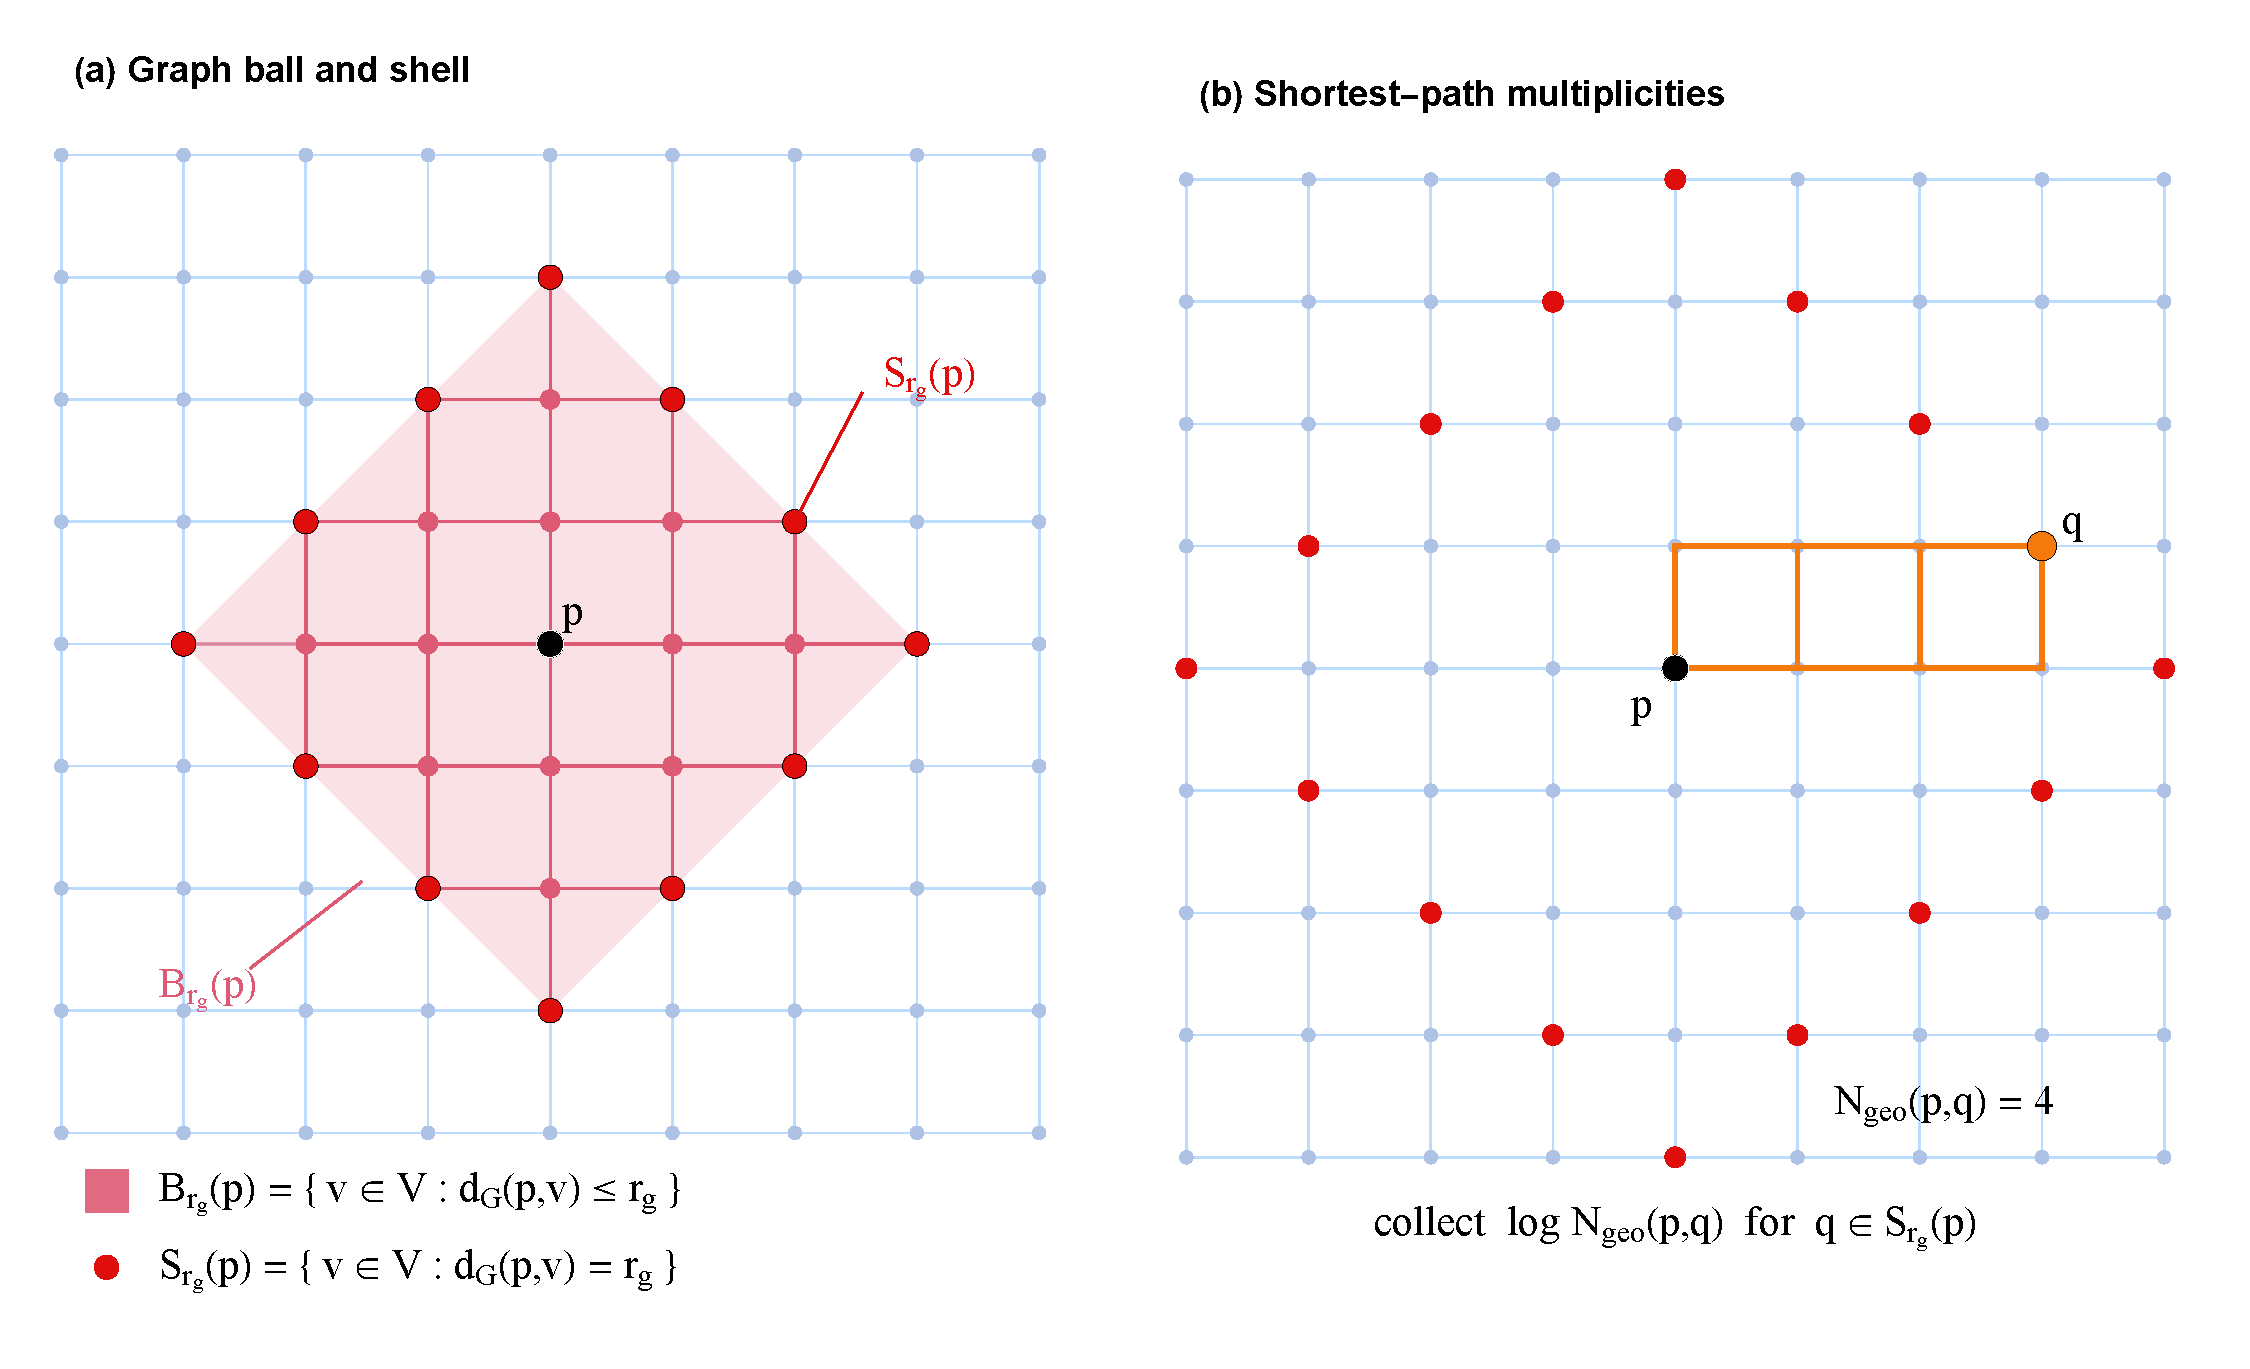
\includegraphics[width=0.9
\textwidth]{results/figures/grid_ball_shell_paths.pdf}
\caption{Schematic of the shell-based shortest-path construction. 
(a) For a source node $p$ and graph radius $r_g$, the graph ball 
$B_{r_g}(p)$ contains all nodes satisfying $d_G(p,v)\le r_g$, while the shell 
$S_{r_g}(p)$ contains only nodes satisfying $d_G(p,v)=r_g$. 
(b) For each target node $q\in S_{r_g}(p)$, we count the number of graph shortest paths 
$N_{\mathrm{geo}}(p,q)$ from $p$ to $q$. The logarithmic multiplicities 
$\log N_{\mathrm{geo}}(p,q)$ over the shell form the distribution used to define 
$C_{\log}(p,r_g)$.}
\label{fig:shell-schematic}
\end{figure}

\subsection{Logarithmic Path-Anisotropy Statistic}

For a fixed source node $p$ and graph radius $r_g$, we collect the logarithmic shortest-path multiplicities
\begin{equation}
X_{p,r_g}=\{\log N_{\mathrm{geo}}(p,q): q\in S_{r_g}(p)\}.
\end{equation}
The logarithm reduces the dominance of unusually high-multiplicity targets and makes the statistic more stable across graph sizes.

We define the logarithmic path-anisotropy statistic as the cubic mean deviation of this shell distribution:
\begin{equation}
C_{\log}(p,r_g)=
\left[\frac{1}{|S_{r_g}(p)|}\sum_{q\in S_{r_g}(p)}
\left|\log N_{\mathrm{geo}}(p,q)-\mu_{p,r_g}\right|^3
\right]^{1/3},
\label{eq:clog}
\end{equation}
where
\begin{equation}
\mu_{p,r_g}=\frac{1}{|S_{r_g}(p)|}\sum_{q\in S_{r_g}(p)}\log N_{\mathrm{geo}}(p,q).
\end{equation}
If $|S_{r_g}(p)|$ is too small, the node is excluded from the analysis for that radius. In practice, this removes boundary nodes and poorly resolved regions.

The statistic $C_{\log}$ is large when shortest-path multiplicities toward the shell are unevenly distributed. It is small when the shell has relatively uniform multiplicity. In a spatial graph, such unevenness may arise from curvature, bottlenecks, sampling irregularity, boundaries, or construction artifacts. The role of the matched-control protocol is to identify which component is systematically associated with the target geometry.

\subsection{Radial Aggregation}

In radially organized benchmark geometries, each node $p$ is assigned a radial coordinate $r(p)$ inherited from the sampled domain. We group nodes into radial bins and compute the mean statistic
\begin{equation}
\overline{C}_{\log}(r_i,r_g)=\frac{1}{|\mathcal{B}_i|}\sum_{p\in\mathcal{B}_i}C_{\log}(p,r_g),
\end{equation}
where $\mathcal{B}_i$ denotes the set of nodes in the $i$th radial bin. The binned profile is then compared to the continuum reference profile, such as $K_{\mathrm{Schw}}(r)$ or $\log K_{\mathrm{Schw}}(r)$ in the Schwarzschild benchmark.

\begin{figure}
\centering
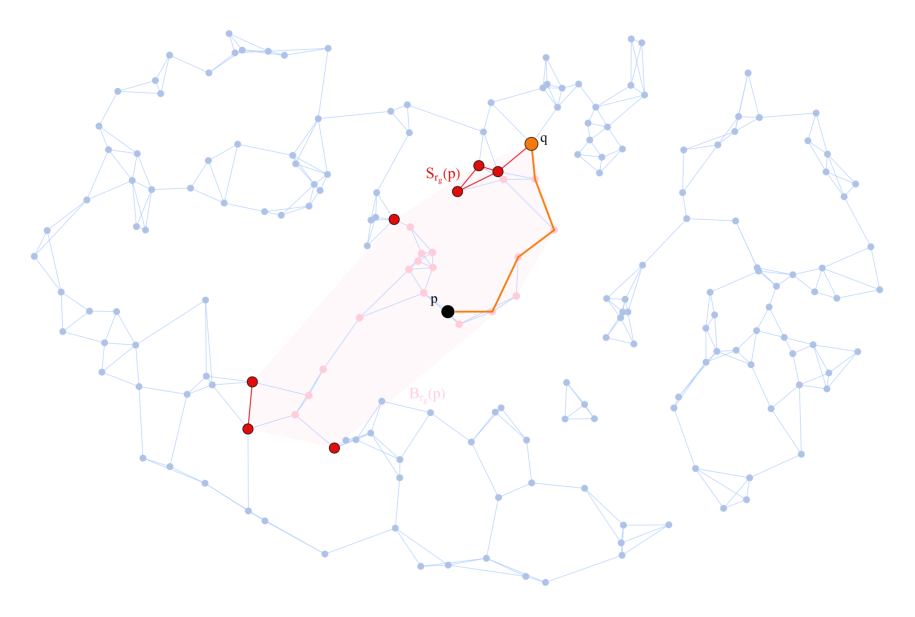
\includegraphics[width=0.8\textwidth]{results/figures/curved_ball_shell_paths_rasterized.pdf}
\caption{Illustration of the same ball-shell construction on an irregular spatial graph sampled from a curved benchmark domain. The source node $p$ defines a local graph ball $B_{r_g}(p)$ and shell $S_{r_g}(p)$, while highlighted paths indicate representative shortest paths from $p$ to a shell target $q$. This schematic emphasizes that the statistic is applied to spatial graph discretizations beyond regular lattice examples.}
\label{fig:curved-shell-schematic}
\end{figure}

\section{Experimental Design}

\subsection{Benchmark Geometries}

We test the statistic on three classes of graph discretizations.

\paragraph{Flat matched controls.}
Flat graphs provide a baseline for the effect of sampling, graph construction, and finite-size variation. These controls are matched to the curved experiments as closely as possible in node number and graph construction.

\paragraph{Hyperbolic controls.}
Hyperbolic geometries serve as non-black-hole curved benchmarks. They test whether the statistic responds to geometric organization beyond a single physical example.

\paragraph{Black-hole-inspired spatial geometries.}
The main benchmark is the Flamm--Schwarzschild spatial slice. This geometry is useful because it has radial structure and a simple continuum curvature reference. We also use charged or regular black-hole-inspired variants, such as Reissner--Nordstr\"om, Bardeen, and Hayward families, as stress tests of the method under changes in the radial geometry.

\subsection{Graph Parameters}

Graphs are generated with fixed random seeds and repeated across multiple resolutions. The main refinement tests use $N=200$, $N=500$, and $N=1000$ sampled nodes. Nearest-neighbor values in the range $k=12,14,16,18,20$ are used to test robustness against graph density. Graph radii $r_g=2,\ldots,7$ are examined to distinguish local and mesoscopic shell behavior.

\begin{table}
\centering
\caption{Summary of the experimental protocol used in the numerical benchmarks. The same graph-construction choices are applied across the curved geometries and matched-flat controls to isolate geometry-related organization from sampling and discretization effects.}
\label{tab:protocol}
\begin{tabular}{ll}
\toprule
Component & Protocol \\
\midrule
Graph type & Spatial nearest-neighbor graphs \\
Node counts & $N=200,500,1000$ \\
Nearest-neighbor values & $k=12,14,16,18,20$ \\
Graph radii & $r_g=2,\ldots,7$ \\
Main benchmark & Flamm--Schwarzschild spatial slice \\
Controls & Matched-flat and hyperbolic graph discretizations \\
Main statistic & $C_{\log}(p,r_g)$ \\
Reference profile & $K_{\mathrm{Schw}}(r)=48M^2/r^6$ \\
\bottomrule
\end{tabular}
\end{table}

\subsection{Evaluation Metrics}

We evaluate the statistic using three complementary criteria.

First, we examine radial profiles of $\overline{C}_{\log}$ and compare them against the expected monotonic radial behavior of the benchmark geometry. Second, we compute correlations between $\overline{C}_{\log}$ and $\log K_{\mathrm{Schw}}$ in the Flamm benchmark. Third, we compare the curved results to matched-flat controls to test whether the observed trend is specific to the curved geometry or merely a consequence of sampling and graph construction.

\section{Results}

\subsection{Shell-Based Anisotropy Detects Radial Organization}

Using the shell-based construction defined in Section 3 and illustrated in Fig.~\ref{fig:shell-schematic}, we compute $C_{\log}(p,r_g)$ for each admissible source node and aggregate the resulting values in radial bins. This allows us to test whether shortest-path multiplicity anisotropy displays systematic radial organization in curved graph discretizations.

In the Flamm--Schwarzschild benchmark, the radial profile of $\overline{C}_{\log}$ decreases with radius in a manner consistent with the decreasing continuum curvature scale. This behavior is absent or much weaker in the matched-flat controls. In the current runs, the correlation between radius and the statistic is approximately
\begin{equation}
\mathrm{Corr}(r,C_{\log})_{\mathrm{Flamm}}=-0.960\pm 0.015,
\end{equation}
whereas the matched-flat control gives
\begin{equation}
\mathrm{Corr}(r,C_{\log})_{\mathrm{MatchedFlat}}=0.180\pm 0.315.
\end{equation}
The large difference between these two values indicates that the statistic is not merely detecting the presence of a radial coordinate or finite sampling, but responds to the organized distortion present in the curved benchmark.


\begin{figure}[t]
    \centering
    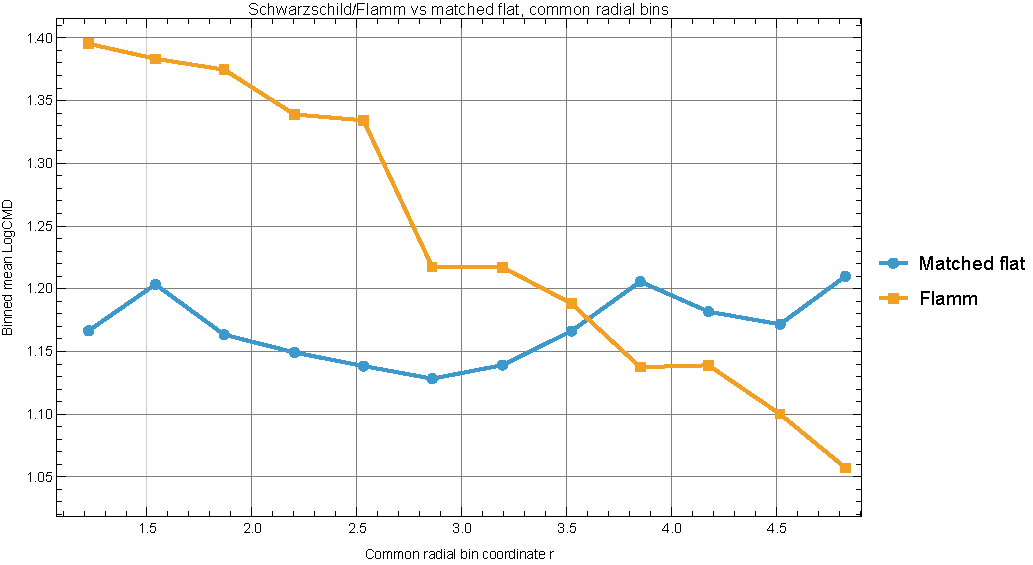
\includegraphics[width=0.75\textwidth]{results/figures/flamm_matched_flat_common_bins.pdf}
    \caption{Radial profiles of the shell-averaged shortest-path anisotropy statistic $\overline{C}_{\log}$ for the Schwarzschild/Flamm benchmark and a matched-flat control, evaluated on common radial bins. The Flamm graph displays a systematic radial decrease in $\overline{C}_{\log}$, whereas the matched-flat control remains comparatively weakly structured. This comparison indicates that the observed radial organization is not reproduced by the matched flat discretization alone.}
    \label{fig:radial-profiles}
\end{figure}

\subsection{Agreement with the Continuum Curvature Profile}

The Flamm--Schwarzschild benchmark allows a direct comparison with a known continuum curvature scale. Although $C_{\log}$ is not a curvature scalar, the binned statistic tracks the radial organization of $\log K_{\mathrm{Schw}}$. In the current radial-binned experiment, we find
\begin{equation}
\mathrm{Corr}\left(\log K_{\mathrm{Schw}},\overline{C}_{\log}\right)\approx 0.912.
\end{equation}
This strong correlation suggests that shortest-path multiplicity anisotropy captures geometry-induced organization in the graph discretization.

\begin{figure}
\centering
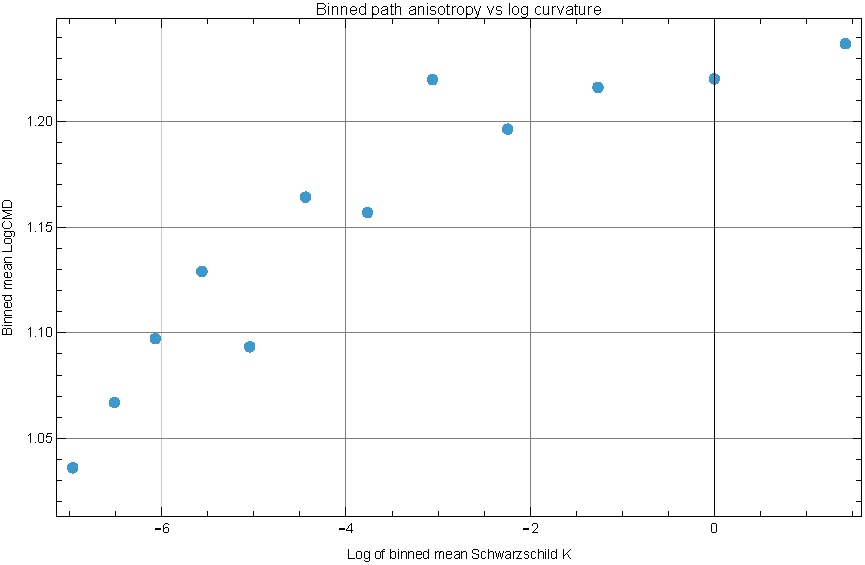
\includegraphics[width=0.85\textwidth]{binned_estimator_vs_logK.pdf}
\caption{Binned path-anisotropy statistic compared with the logarithmic Schwarzschild reference profile $\log K_{\mathrm{Schw}}$. The observed correlation is approximately $0.912$ in the current Flamm benchmark.}
\label{fig:logK}
\end{figure}

\subsection{Resolution Dependence}

A useful graph diagnostic should improve or stabilize as the discretization is refined. Table~\ref{tab:refinement} shows the mean rank agreement across the refinement sequence used in the current experiments. The Spearman correlation increases from $N=200$ to $N=1000$, suggesting that the statistic becomes more stable as the sampled geometry is better resolved.

\begin{table}
\centering
\caption{Resolution dependence of the rank agreement between the graph diagnostic and the continuum reference profile in the Flamm benchmark. The increase in agreement with $N$ suggests improved stability under refinement, although larger ensembles are needed to establish a convergence trend.}
\label{tab:refinement}
\begin{tabular}{cc}
\toprule
Number of sampled nodes & Mean Spearman agreement \\
\midrule
$N=200$ & $0.5320$ \\
$N=500$ & $0.5630$ \\
$N=1000$ & $0.6636$ \\
\bottomrule
\end{tabular}
\end{table}

The increase is not presented as a convergence theorem. Rather, it provides empirical support that the statistic is resolving a geometric signal rather than purely finite-sample noise. Larger ensembles are still needed to establish a systematic convergence trend.

\subsection{Robustness Across Graph Radius and Density}

We also test the dependence of the statistic on graph radius $r_g$ and nearest-neighbor parameter $k$. The signal remains qualitatively stable across $k=12,14,16,18,20$ and $r_g=2,\ldots,7$. Smaller graph radii probe more local shell structure, while larger radii include more mesoscopic organization but are more sensitive to boundaries and finite-size effects. In practice, the most useful regime is an intermediate graph radius where shells contain enough nodes for a stable dispersion statistic while remaining sufficiently local to track radial structure.

\begin{figure}
\centering
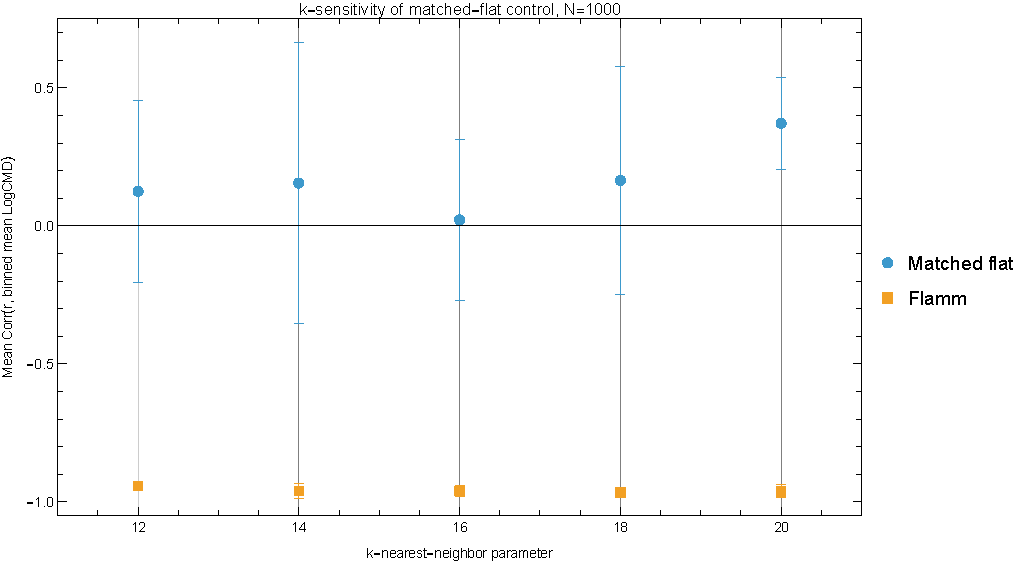
\includegraphics[width=0.9\textwidth]{k_sensitivity_matched_flat_flamm_N1000_errors.pdf}
\caption{Sensitivity of the radial correlation $\mathrm{Corr}(r,\overline{C}_{\log})$ to the $k$-nearest-neighbor parameter for $N=1000$. Error bars summarize variation across the tested graph radii $r_g=2,\ldots,7$. The Flamm benchmark remains strongly negative across the tested values of $k$, while the matched-flat control fluctuates around weaker correlations.}
\label{fig:robustness}
\end{figure}

\section{Discussion}

The experiments support the interpretation of $C_{\log}$ as a curvature-sensitive diagnostic for spatial graph discretizations. The key point is not that the statistic equals a continuum curvature invariant. It does not. Instead, the statistic detects how the distribution of shortest-path degeneracies changes across a graph sampled from a radially organized geometry. In the Flamm--Schwarzschild benchmark, this change aligns strongly with the continuum radial curvature profile after radial binning.

The matched-flat controls are essential. Without them, a radial trend in $C_{\log}$ could be dismissed as a sampling artifact or boundary effect. The observed difference between the Flamm benchmark and the matched-flat controls indicates that the signal is tied to the geometric distortion of the curved sample, at least under the graph-construction protocol used here.

The method also offers a useful complement to local graph-curvature measures. Forman--Ricci and Ollivier--Ricci curvature assign curvature-like values to edges or nodes based on local combinatorial or transport structure. By contrast, $C_{\log}$ is shell-based and path-multiplicity based. It probes how families of shortest paths distribute around a source node. This makes it sensitive to mesoscopic geometry and anisotropy rather than only local edge structure.

At the same time, the method has clear limitations. First, it depends on the graph-construction rule. Changing from a $k$-nearest-neighbor graph to a radius graph, weighted graph, or Delaunay-type construction may change the statistic. Second, it depends on sampling quality. Strongly nonuniform sampling can create artificial anisotropy unless matched controls or density corrections are used. Third, graph boundaries can distort shells and path multiplicities. Boundary filtering is therefore necessary. Fourth, the current comparison is empirical; a theoretical relationship between path-multiplicity anisotropy and continuum curvature remains open.

These limitations are not defects of the method so much as constraints on its interpretation. We propose $C_{\log}$ as a calibrated diagnostic for graph discretizations, not as a universal curvature scalar. Under that interpretation, the statistic is useful because it is simple, computable from unweighted graph topology, and responsive to geometric organization in controlled benchmarks.

\section{Conclusion}

We introduced a shell-based shortest-path anisotropy statistic for spatial graphs sampled from geometric domains. The statistic measures the logarithmic dispersion of shortest-path multiplicities from a source node to a fixed graph shell. Applied to flat, hyperbolic, and black-hole-inspired graph discretizations, the method detects radial organization in curved benchmarks while matched-flat controls do not reproduce the same systematic trend. In the Flamm--Schwarzschild case, the binned statistic correlates strongly with the continuum reference profile $\log K_{\mathrm{Schw}}$.

The results suggest that shortest-path anisotropy is a promising network diagnostic for geometry-sensitive analysis of spatial graphs. Future work will extend the method to weighted graphs, alternative graph constructions, more benchmark manifolds, and comparisons with local graph-curvature measures. A theoretical characterization of when path-multiplicity anisotropy reflects continuum curvature remains an important open problem.

\begingroup
\hbadness=10000
\begin{thebibliography}{99}

\bibitem{Ollivier2009}
Ollivier, Y.: Ricci curvature of Markov chains on metric spaces. Journal of Functional Analysis 256(3), 810--864 (2009)

\bibitem{Forman2003}
Forman, R.: Bochner's method for cell complexes and combinatorial Ricci curvature. Discrete \& Computational Geometry 29, 323--374 (2003)

\bibitem{Ni2019}
Ni, C.-C., Lin, Y.-Y., Luo, F., Gao, J.: Community detection on networks with Ricci flow. Scientific Reports 9, 9984 (2019)

\bibitem{Sandhu2015}
Sandhu, R., Georgiou, T., Tannenbaum, A.: Ricci curvature: An economic indicator for market fragility and systemic risk. Science Advances 2(5), e1501495 (2016)

\bibitem{Penrose1972}
Penrose, R.: Techniques of Differential Topology in Relativity. SIAM, Philadelphia (1972)

\bibitem{Schwarzschild1916}
Schwarzschild, K.: On the gravitational field of a mass point according to Einstein's theory. Sitzungsberichte der K\"oniglich Preussischen Akademie der Wissenschaften, 189--196 (1916)

\bibitem{Flamm1916}
Flamm, L.: Beitr\"age zur Einsteinschen Gravitationstheorie. Physikalische Zeitschrift 17, 448--454 (1916)

\bibitem{Newman1999}
Newman, M.E.J., Watts, D.J.: Scaling and percolation in the small-world network model. Physical Review E 60, 7332--7342 (1999)

\bibitem{Barabasi2016}
Barab\'asi, A.-L.: Network Science. Cambridge University Press, Cambridge (2016)

\bibitem{Krioukov2010}
Krioukov, D., Papadopoulos, F., Kitsak, M., Vahdat, A., Bogu\~n\'a, M.: Hyperbolic geometry of complex networks. Physical Review E 82, 036106 (2010)

\end{thebibliography}
\endgroup

\end{document}
